\documentclass[12pt]{article}

\usepackage[margin=0.45in]{geometry}
\usepackage{amsmath,amssymb}
\usepackage{booktabs}
\usepackage{graphicx}
\usepackage{url}
\usepackage{array}
\usepackage{titlesec}
\usepackage{float}

\setlength{\parskip}{0pt}
\setlength{\floatsep}{6pt plus 1pt minus 1pt}
\setlength{\textfloatsep}{6pt plus 1pt minus 1pt}
\setlength{\intextsep}{6pt plus 1pt minus 1pt}
\setlength{\abovedisplayskip}{5pt plus 1pt minus 1pt}
\setlength{\belowdisplayskip}{5pt plus 1pt minus 1pt}
\titlespacing*{\section}{0pt}{0.75ex plus 0.2ex minus 0.1ex}{0.35ex plus 0.1ex}

\title{\vspace{-1.1em}Geometry-Aware Joint Set Transformer for Billiards Break Prediction}
\author{Bu Yizhe \quad Tang Wentao \quad Wang Mingyang}
\date{}

\begin{document}
\maketitle
\vspace{-1.4em}

\begin{abstract}
Break-shot prediction from a post-break table state is a compact physical reasoning problem: the input is an unordered scene of balls and pockets, and the outputs are coupled events rather than independent labels.  This report studies that mismatch directly.  BLFormer represents the layout as a variable-size object set, injects pairwise billiards geometry into self-attention, and predicts a joint 40-state outcome distribution whose marginals produce clear, win, and potted-count predictions.  Against BLCNN, MLP, and vanilla Transformer baselines on the same held-out protocol, the selected BLFormer reaches 71.82\% clear accuracy, 69.67\% win accuracy, and 67.10\% potted-count accuracy, with the largest gain on the count prediction task.
\end{abstract}
\vspace{-0.7em}

\section{Introduction}
The prediction task asks a simple question: given the observed layout after a break shot, can we predict whether the rack will be cleared, whether the player will win, and how many balls are potted?  A useful model must resolve two forms of structure.  First, the layout is not an image with a stable raster semantics; it is a set of physical objects whose pairwise routes, angles, and occlusions matter.  Second, the labels are coupled: a state that makes many balls available changes both clear and win probabilities.  Standard baselines address only part of this structure: BLCNN operates on paper-style layout tokens, MLP flattens the same information, and a vanilla Transformer attends over tokens without billiards-specific relational bias.

BLFormer is designed around these two mismatches.  It treats active balls and pockets as tokens, uses geometric pair features as attention bias, and replaces independent prediction with a joint outcome head.  The objective of this report is not to reproduce historical paper-table numbers; it is to give a clean held-out comparison of these modeling choices under one protocol, with all selection performed inside the training partition.

\section{Dataset and Preprocessing}
The dataset contains 1,940 accepted post-break table states: 776 for training and 1,164 for held-out testing.  For model-family selection, the training layouts are split into 660 internal training samples and 116 validation samples.  The input is the observed table state after the break; balls already potted during the break are therefore absent and may be masked.  The labels describe downstream outcomes from that state: clear, win, and potted count.  This is important: the setup is a post-break-state predictor, not a pre-impact predictor.

Preprocessing is kept explicit because small changes in this dataset can alter conclusions.  Spreadsheets are aligned to coordinate XML files by frame.  Rows are removed when labels are outside valid ranges, remarks contain cue-ball/foul/illegal/golden-break markers, the XML does not contain exactly ten markers, or the normalized layout duplicates an earlier accepted sample.  Duplicate keys are rounded normalized ball features at four decimals.  Coordinates are mapped to a 200-by-100 table: files with the long axis stored first use $(x/200,y/100)$, otherwise axes are swapped; values are clamped to $[0,1]$ to remove out-of-table artifacts.  Balls potted during the break receive existence zero and coordinates $(0,0)$ so they are not obstacles.  Each packed ball feature is
\[
  x_b = [x_b^{norm}, y_b^{norm}, \mathbb{1}_{exists}, b/9].
\]
At training time, BLFormer converts only active balls to tokens, appends six fixed pocket tokens, and pads batches with an attention mask.  Horizontal and vertical flips are applied independently with probability 0.5 only to training layouts; this preserves table symmetries without changing labels.  No augmentation is applied to validation or test data.  No resampling is used: the held-out distribution is kept natural, while imbalance is monitored through rare-class analysis and addressed through joint and marginal supervision.  Label counts are clear 994/946, win 607/1333, and potted counts $[739,110,58,44,28,29,96,381,451,4]$ for classes 0--9.

\section{Method}
BLFormer has two design commitments: relational scene encoding and joint label modeling.  The encoder follows the Set Transformer view that unordered inputs should be processed as sets \cite{lee2019set}, but it also uses the table geometry that ordinary attention would have to rediscover from few samples.  Following Graphormer-style structural bias \cite{ying2021graphormer}, pair features are mapped to an additive attention bias in every layer.  This lets the model attend with knowledge of distance, direction, pocket route, and obstruction while still learning task-specific representations.

For tokens $i,j$, the 10-dimensional pair vector $\phi_{ij}$ contains normalized distance, $\Delta x$, $\Delta y$, a task-specific angle feature, a blocked-path indicator, and a four-way edge type one-hot code for CLS/pad, ball-ball, ball-pocket, and pocket-pocket edges.  Multi-head attention is computed as
\[
  \alpha_{ij}^{(h)}
  = \mathrm{softmax}_j\left(
      \frac{q_i^{(h)\top} k_j^{(h)}}{\sqrt{d_h}}
      + f_h(\phi_{ij}) + m_j
    \right),
\]
where $f_h$ is a two-layer MLP producing one scalar bias per head and $m_j$ masks padding.  Each encoder block uses pre-normalization, residual attention, and a GELU feed-forward network.  Token embeddings combine type, ball identity, and coordinates.  The pooled layout representation concatenates the CLS token with the mean over valid tokens, reducing dependence on a single summary token.

The potted-count target is evaluated as exact 10-class accuracy, and its empirical distribution is multimodal, with dominant modes at 0, 7, and 8.  The selected model therefore treats potted count as a categorical marginal of a stronger joint outcome model rather than as an independent count regressor.  The joint head predicts one of $2\times2\times10=40$ states:
\[
  c = 20\,y_{clear} + 10\,y_{win} + y_{pot}.
\]
Task logits are recovered by marginalizing the 40 logits with log-sum-exp, e.g.
\[
  s_{clear} =
  \log\sum_{w,p}\exp g_{1,w,p}
  - \log\sum_{w,p}\exp g_{0,w,p}.
\]
The potted-count logits are recovered analogously as
\[
  s_{pot}(p)=\log\sum_{c,w}\exp g_{c,w,p}.
\]
This head explicitly models outcome correlation: a state favorable for potting many balls should also affect clear and win probabilities.  The selected model uses joint cross-entropy as the main objective and a smaller marginal auxiliary objective:
\[
  \mathcal{L}= \mathrm{CE}(g,c)
  + 0.5\,(\mathcal{L}_{clear}+\mathcal{L}_{win}+\mathcal{L}_{pot})/3.
\]
Here $\mathcal{L}_{clear}$ and $\mathcal{L}_{win}$ are binary cross-entropies on the marginalized clear and win logits, and $\mathcal{L}_{pot}$ is 10-class cross-entropy on the marginalized potted-count logits.

\section{Training and Metrics}
All experiments use the same deterministic split protocol.  BLFormer is trained with AdamW, learning rate $3\times10^{-4}$, weight decay 0.01, batch size 64, cosine annealing, dropout 0.1, gradient clipping at 1.0, and early stopping with patience 60 over at most 400 epochs.  Hidden width is searched over $d\in\{64,80,88\}$ and selected on the internal validation split by a three-task balance criterion: the configuration must maximize the weakest validation margin across clear, win, and potted-count accuracy, rather than using held-out test performance.  The selected joint model uses width 80, two encoder layers, four attention heads, CLS+mean pooling, and 121,426 parameters.  We report accuracy for each task and mean accuracy; macro-F1 and potted-count MAE are used for error analysis.

\section{Experiments and Results}
Table~\ref{tab:results} is organized to answer a progression of questions.  First, how strong are standard baselines on the same held-out split?  BLCNN is a convolutional baseline over paper-style layout tokens, MLP is a flattened token baseline, and Transformer is a vanilla token baseline without BLFormer geometry bias or joint outcome modeling.  Second, does the BLFormer representation help once the three tasks are predicted together?  Third, does explicit joint supervision help over independent heads?  Baselines are trained per task for 400 epochs; BLFormer rows use internal validation within the training partition.

The selected BLFormer obtains 69.53\% mean accuracy, compared with 66.49\% for the strongest baseline mean.  The largest difference is on potted-count prediction, where BLFormer reaches 67.10\% versus 61.25\% for BLCNN, 55.24\% for MLP, and 40.12\% for the vanilla Transformer.  The reported result uses the model selected by internal validation, keeping the comparison tied to the training protocol.

\begin{table}[H]
\centering
\setlength{\tabcolsep}{2pt}
\caption{Held-out test comparison across baseline methods and BLFormer variants. Bold indicates the best value in each metric column.}
\label{tab:results}
\begin{tabular}{lrrrr}
\toprule
Model family & Clear & Win & Potted & Mean \\
\midrule
BLCNN baseline & 71.48 & 66.75 & 61.25 & 66.49 \\
MLP baseline & 69.33 & 67.18 & 55.24 & 63.92 \\
Transformer baseline & 65.81 & 66.41 & 40.12 & 57.45 \\
Independent-head BLFormer & 69.42 & \textbf{70.45} & 65.81 & 68.56 \\
Joint-outcome BLFormer & 70.96 & 70.19 & 66.92 & 69.36 \\
Joint-outcome BLFormer with auxiliary loss & \textbf{71.82} & 69.67 & \textbf{67.10} & \textbf{69.53} \\
\bottomrule
\end{tabular}
\end{table}

\begin{figure}[H]
  \centering
  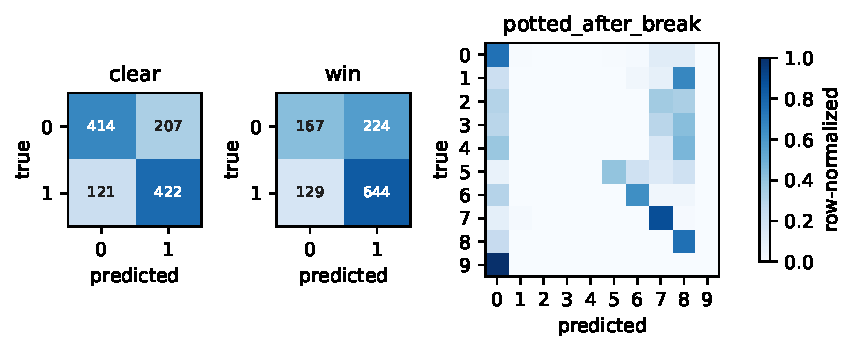
\includegraphics[width=0.78\linewidth]{figures/confusion_matrices.pdf}
  \caption{Held-out confusion matrices for the selected joint model.  The potted-count head is accurate on dominant classes but weak on rare counts.}
  \label{fig:confusion}
\end{figure}

\section{Analysis and Limitations}
The comparison suggests that the main benefit is not simply more capacity.  The best independent BLFormer improves mean accuracy over BLCNN, but the joint head moves the model further by sharing information across correlated outcomes.  Auxiliary marginal supervision then improves clear from 70.96\% to 71.82\% and potted count from 66.92\% to 67.10\%, with a moderate win trade-off.  This supports the selected design, while still leaving component-level geometry ablations for future work.

The dominant failure mode is long-tail potted-count behavior.  Although exact potted accuracy is 67.10\%, macro-F1 is only 0.338.  The selected model predicts mostly classes 0, 7, and 8 and never predicts class 9 on the held-out set; the potted mean absolute error is 2.05 balls, with 69.07\% of predictions within one ball.  Figure~\ref{fig:confusion} makes this concentration visible.  Win is also noisy, with many false positives because the positive class is dominant.  The final limitation is reproducibility granularity: the report uses one fixed split and deterministic training run, so future work should add multi-seed confidence intervals and calibration analysis for rare potted classes.

\section{Conclusion}
The report frames billiards break prediction as relational scene understanding with coupled labels.  BLFormer follows that framing by combining object-set encoding, geometry-biased attention, and joint outcome supervision.  Under the held-out protocol, the validation-selected joint model achieves the strongest reported result: 71.82\% clear, 69.67\% win, and 67.10\% potted-count accuracy.  The remaining weakness is not the average score but rare-count behavior, which points to calibration and multi-seed evaluation as the next improvements.

\section{Author Contributions}
Bu Yizhe worked on the MLP baseline, result organization, and evaluation.  Tang Wentao worked on BLFormer and the Transformer baseline.  Wang Mingyang worked on preprocessing and the BLCNN baseline.

\begin{thebibliography}{9}
\bibitem{ying2021graphormer}
Chengxuan Ying, Tianle Cai, Shengjie Luo, Shuxin Zheng, Guolin Ke, Di He, Yanming Shen, and Tie-Yan Liu.
\newblock Do Transformers Really Perform Bad for Graph Representation?
\newblock \emph{NeurIPS}, 2021. \url{https://arxiv.org/abs/2106.05234}.

\bibitem{lee2019set}
Juho Lee, Yoonho Lee, Jungtaek Kim, Adam R. Kosiorek, Seungjin Choi, and Yee Whye Teh.
\newblock Set Transformer: A Framework for Attention-based Permutation-Invariant Neural Networks.
\newblock \emph{ICML}, 2019. \url{https://arxiv.org/abs/1810.00825}.

\end{thebibliography}

\end{document}
